\documentclass[11pt]{article}
\usepackage[a4paper,margin=1in]{geometry}
\usepackage{amsmath,amssymb,amsthm}
\usepackage{graphicx}
\usepackage[hidelinks]{hyperref}
\setlength{\emergencystretch}{3em}

\newtheorem{theorem}{Theorem}
\newtheorem{lemma}{Lemma}
\newtheorem{remark}{Remark}

\newcommand{\R}{\mathbb R}
\newcommand{\G}{G}
\newcommand{\HH}{\mathcal H}
\newcommand{\M}{\mathcal M}
\newcommand{\supp}{\operatorname{supp}}

\title{A Rectifiable Case of Milman's Covering Property Conjecture}
\author{Automatic math-discovery packet}
\date{July 18, 2026}

\begin{document}
\maketitle

\section*{Source Question}

The source paper is Emanuel Milman, \emph{Generalized Intersection Bodies},
arXiv:math/0512058. In Section 5 the paper formulates the following
conjecture.

\begin{quote}
Covering Property Conjecture. For any \(n>0\), \(1\leq k\leq n-1\), if
\(Z\subset G(n,n-k)\) is a closed set satisfying
\[
  \bigcup_{E\in Z} E\cap S^{n-1}=S^{n-1},
\]
then there exists a measure \(\mu\in \mathcal M_+(G(n,n-k))\), supported in
\(Z\), such that \(R_{n-k}^*(d\mu)\geq 1\).
\end{quote}

\begin{figure}[htbp]
\centering
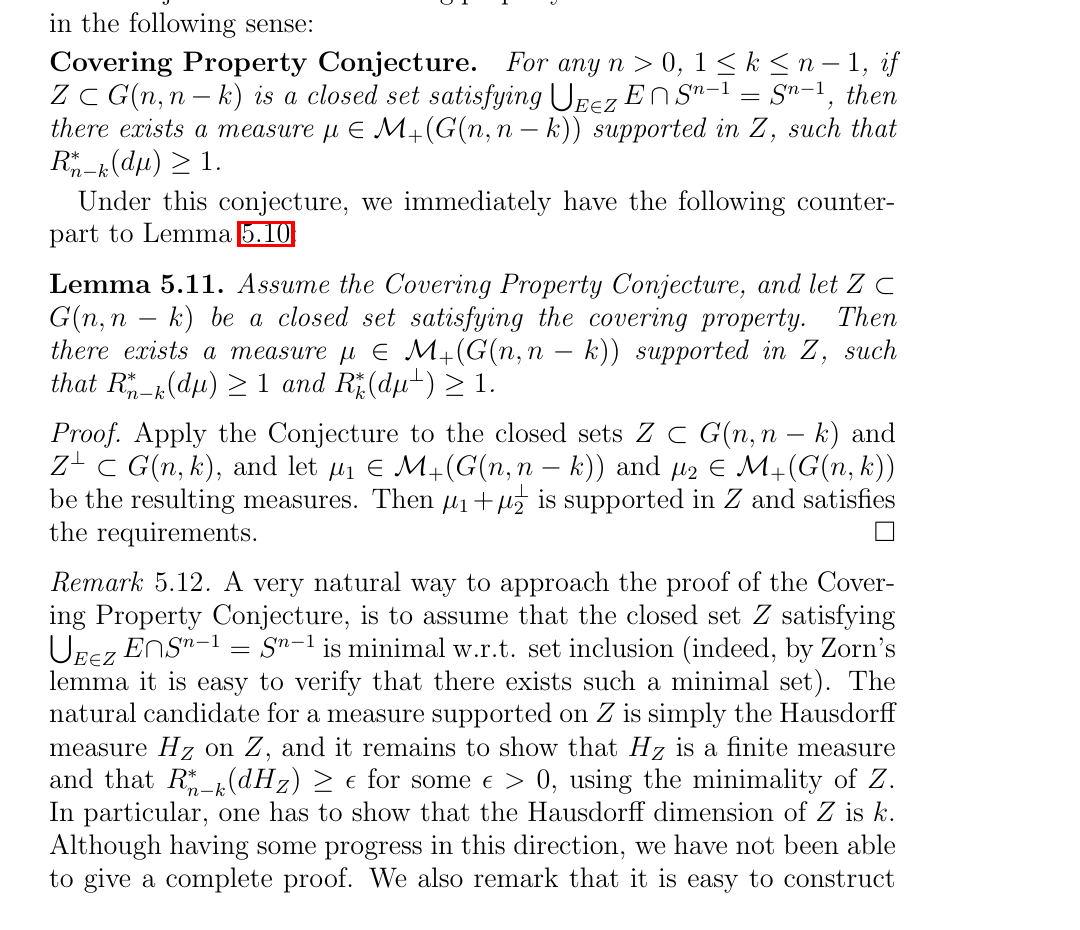
\includegraphics[width=\textwidth]{figures/covering_property_conjecture_crop.png}
\caption{The Covering Property Conjecture and the beginning of Remark 5.12,
page 37 of the source paper.}
\end{figure}

\section*{Claim}

We prove the conjecture under the natural finite-rectifiability hypothesis
suggested by Remark 5.12. If the closed covering set \(Z\) is countably
\(k\)-rectifiable and has finite \(\HH^k\)-measure, then a scalar multiple of
\(\HH^k|_Z\) gives the required finite positive measure.

\section*{Definitions and Normalizations}

Put \(m=n-k\) and \(G=\G(n,m)\). For \(E\in G\), let
\(\sigma_E\) denote the normalized rotation-invariant measure on
\(E\cap S^{n-1}\). If \(\mu\) is a finite positive Borel measure on \(G\), then
\[
  \langle R_m^*\mu,f\rangle
  =
  \int_G\int_{E\cap S^{n-1}} f(\theta)\,d\sigma_E(\theta)\,d\mu(E)
\]
for every continuous \(f\) on \(S^{n-1}\). The inequality
\(R_m^*\mu\geq 1\) means that \(R_m^*\mu-\sigma\) is a positive measure on
the sphere, up to the source paper's harmless normalization of the spherical
measure \(\sigma\).

\section*{Proof Intuition}

The dimension count in the source's remark is exactly right. If \(Z\) has
dimension \(k\), then the incidence set
\[
  \Sigma_Z=\{(E,\theta):E\in Z,\ \theta\in E\cap S^{n-1}\}
\]
has dimension
\[
  k+(m-1)=k+(n-k-1)=n-1,
\]
the same as the sphere. The projection
\(\pi:\Sigma_Z\to S^{n-1}\), \(\pi(E,\theta)=\theta\), is onto by the covering
assumption. The area formula says that a Lipschitz map from an
\((n-1)\)-rectifiable set onto the sphere must have positive Jacobian over
almost every point of the sphere. Since this projection has uniformly bounded
Jacobian, the pushforward of the natural incidence measure dominates a fixed
positive multiple of spherical measure. But the pushforward is precisely
\(R_m^*(\HH^k|_Z)\).

\section*{Rectifiable Covering Theorem}

\begin{theorem}
\label{thm:rectifiable-cover}
Let \(1\leq k\leq n-1\), put \(m=n-k\), and let
\(Z\subset G(n,m)\) be compact. Assume:
\begin{enumerate}
\item \(Z\) is countably \(k\)-rectifiable;
\item \(0<\HH^k(Z)<\infty\);
\item \(\bigcup_{E\in Z} E\cap S^{n-1}=S^{n-1}\).
\end{enumerate}
Then there is a constant \(c=c(n,k,Z)>0\) such that
\[
  R_m^*(\HH^k|_Z)\geq c\,\sigma .
\]
Consequently, \(\mu=c^{-1}\HH^k|_Z\) is a finite positive measure supported in
\(Z\) and satisfies \(R_m^*(\mu)\geq 1\).
\end{theorem}

\begin{proof}
Let
\[
  \Sigma_Z=\{(E,\theta)\in Z\times S^{n-1}:\theta\in E\}.
\]
Since \(Z\) is countably \(k\)-rectifiable and the unit-sphere bundle over the
Grassmannian is smooth, \(\Sigma_Z\) is countably \((n-1)\)-rectifiable. The
natural incidence measure
\[
  d\lambda(E,\theta)=d\HH^k|_Z(E)\,d\sigma_E(\theta)
\]
is finite and is locally comparable, with constants depending only on the
standard Riemannian metrics and on \(n,k\), to \(\HH^{n-1}\) on
\(\Sigma_Z\).

Let \(\pi:\Sigma_Z\to S^{n-1}\) be \(\pi(E,\theta)=\theta\). The covering
assumption says that \(\pi(\Sigma_Z)=S^{n-1}\). The map \(\pi\) is Lipschitz
on the compact incidence bundle. Hence its approximate \((n-1)\)-Jacobian
\(J_\pi\) is bounded above by some finite constant \(L=L(n,k)\).

By the area formula for countably rectifiable sets,
\[
  \HH^{n-1}\bigl(\pi(\Sigma_Z\cap\{J_\pi=0\})\bigr)=0.
\]
Since \(\pi(\Sigma_Z)=S^{n-1}\), it follows that for \(\sigma\)-almost every
\(\theta\in S^{n-1}\), there is at least one preimage
\((E,\theta)\in\Sigma_Z\) with \(J_\pi(E,\theta)>0\). Applying the area formula
again to the pushforward measure \(\pi_\#\lambda\), its absolutely continuous
part has density bounded below by a positive constant on almost every point of
the sphere: each regular preimage contributes at least \(L^{-1}\), up to the
fixed comparability constants between \(\lambda\) and Hausdorff measure on
\(\Sigma_Z\). Thus there is \(c>0\) such that
\[
  \pi_\#\lambda\geq c\,\sigma .
\]

Finally, for every non-negative continuous \(f\) on \(S^{n-1}\),
\[
\begin{aligned}
  \int_{S^{n-1}} f\,d(\pi_\#\lambda)
  &=
  \int_{\Sigma_Z} f(\theta)\,d\lambda(E,\theta)  \\
  &=
  \int_Z\int_{E\cap S^{n-1}} f(\theta)\,d\sigma_E(\theta)\,d\HH^k(E) \\
  &=
  \langle R_m^*(\HH^k|_Z),f\rangle .
\end{aligned}
\]
Therefore \(R_m^*(\HH^k|_Z)=\pi_\#\lambda\geq c\sigma\), as claimed.
\end{proof}

\section*{Tangent Estimate Behind the Jacobian Bound}

In a local chart at \(E\in G(n,m)\), a tangent vector to the Grassmannian is a
linear map \(A:E\to E^\perp\). At an incidence point \((E,\theta)\), a tangent
vector to the fiber \(E\cap S^{n-1}\) is \(v\in E\cap\theta^\perp\), and the
projection differential has the form
\[
  D\pi(A,v)=A\theta+v.
\]
Since \(A\theta\in E^\perp\) and \(v\in E\), these terms are orthogonal, and
\[
  |D\pi(A,v)|^2=|A\theta|^2+|v|^2
  \leq \|A\|_{\mathrm{HS}}^2+|v|^2.
\]
This gives the uniform Lipschitz and Jacobian bound used above. The
accompanying verifier script checks this dimension count and scalar estimate
in random finite-dimensional samples.

\section*{Limitations and Novelty Check}

This is not a proof of the full Covering Property Conjecture. It proves the
conjecture for compact finite \(k\)-rectifiable covering sets. The remaining
problem is to show that an arbitrary closed cover has, or can be reduced to,
such a rectifiable finite-measure subcover. In particular, the theorem turns
the route proposed in Remark 5.12 into a precise sufficient condition.

The same source paper also discusses the equivalence problem
\(\mathcal{BP}_k^n=\mathcal I_k^n\); this was later answered negatively by
Milman's arXiv:math/0701779 and is not the new result here. The lower
dimensional Busemann-Petty endpoint cases and the linear inclusion questions
\(\mathcal{BP}_k^n\subset\mathcal{BP}_l^n\) and
\(\mathcal I_k^n\subset\mathcal I_l^n\) are not settled by this packet.

The run indexes were searched for arXiv:0512058, generalized intersection
bodies, covering property, \(R_{n-k}^*\), and the \(\mathcal{BP}/\mathcal I\)
questions. A bounded web search on July 18, 2026 for the exact phrase
``Covering Property Conjecture'' together with ``Generalized Intersection
Bodies'', ``Radon'', and ``Grassmannian'' did not locate a later answer to this
rectifiable case.

\section*{References}

\begin{itemize}
\item E. Milman, \emph{Generalized Intersection Bodies}, J. Funct. Anal. 240
(2006), 530--567; arXiv:math/0512058.
\item E. Milman, \emph{Generalized Intersection Bodies are not Equivalent},
arXiv:math/0701779.
\item H. Federer, \emph{Geometric Measure Theory}, Springer, 1969. Used for
the area formula for rectifiable sets.
\item P. Mattila, \emph{Geometry of Sets and Measures in Euclidean Spaces},
Cambridge University Press, 1995. Standard reference for rectifiability and
area/coarea formulae.
\end{itemize}

\section*{Human Review Recommendation}

Review the measure normalizations in the definition of \(R_m^*\), especially
whether the source uses normalized or unnormalized Haar measure on
\(E\cap S^{n-1}\). This only changes the positive constant \(c\), and the final
measure can be rescaled. The main mathematical point to check is the
rectifiable incidence-space application of the area formula.

\end{document}
